\usepackage[T2A]{fontenc}
\usepackage{pscyr}
\usepackage[cp1251]{inputenc}

\usepackage{lscape}

\pagestyle{empty}

\newcounter{slide}

\newcommand{\slide}{
    \stepcounter{slide}
    \fbox{\includegraphics[page=\theslide,width=0.65\textwidth]{../Slides/Bezborodov_Presentation_Parallel_implementation_of_the_ellipsoids_method_for_optimization_problems_of_large_dimension.pdf}}
}

\newcommand{\page}{
    \begin{table}[h!]
        \centering
        \begin{tabular}{cc}
        \slide & \slide
        \end{tabular}
    \end{table}
    \begin{table}[h!]
        \centering
        \begin{tabular}{p{0.8\textwidth}}
        \\
        \\ \hline
        \\
        \\ \hline
        \\
        \\ \hline
        \\
        \\ \hline
        \end{tabular}
    \end{table}
    \newpage
}